% Team convention (paper-bell, research/admet): preprint form in the style of Suleman 2026. Every numbered statement is traced to its
% verifier claims in Appendix C (claim ids from projects/expressivity/paper_evidence.json). Built by expressivity/write_paper.py.
\documentclass[10pt,twocolumn,a4paper]{article}
\usepackage{fontspec}\setmainfont{STIX Two Text}
\usepackage{amsmath,amssymb}\usepackage{unicode-math}\setmathfont{STIX Two Math}
\usepackage[english]{babel}
\usepackage[a4paper,top=22mm,bottom=24mm,left=17mm,right=17mm,columnsep=7mm]{geometry}
\usepackage{booktabs,longtable,array,calc,graphicx,microtype,fancyhdr,xcolor}
\usepackage[hidelinks]{hyperref}
\providecommand{\tightlist}{\setlength{\itemsep}{0pt}\setlength{\parskip}{0pt}}
\pagestyle{fancy}\fancyhf{}
\fancyhead[L]{\small Preprint (2026)}\fancyhead[R]{\small Team Ninja Turtles: Householder complexity of state tracking}
\fancyfoot[C]{\small\thepage}\renewcommand{\headrulewidth}{0pt}
\fancypagestyle{first}{\fancyhf{}\fancyfoot[C]{\small\thepage}}
\begin{document}\thispagestyle{first}
\twocolumn[{%
\noindent{\small Preprint}\\[-1pt]{\small Machine Learning; Computational Complexity}\\[14pt]
\begin{center}{\LARGE\bfseries How Many Householders Does State Tracking Need? An Exact Law for One-Layer Linear RNNs That Circuit Complexity Does Not Predict}\\[12pt]{\large Team Ninja Turtles}\\[3pt]{\small Hack-Nation 2026, Challenge 3 (Agentic Scientific Discovery)}\\[8pt]{\small Preprint, October 2026}\end{center}
\vspace{6pt}\begin{quote}\small\noindent\textbf{Abstract}\enspace The usual account of why architectures fail at state tracking comes from circuit complexity. Log-precision Transformers can be simulated by constant-depth threshold circuits, and SSMs ``cannot express computation outside the complexity class \(\mathsf{TC}^0\)'' {[}C-lit-merrill-tc0{]}{[}C-lit-illusion{]}. We study one-layer linear RNNs whose token transitions are products of generalized Householder factors, as in DeltaNet and DeltaProduct {[}C-lit-deltaproduct{]}{[}C-H-protocol{]}. Consider finite-state realisations of the word problem of a finite group G with alphabet Σ. A finite-state realisation with k factors per token exists if and only if k ≥ \(h^*\)(G, Σ), where \(h^*\) is a group invariant (proved by hand) {[}C-thm1{]}. The lower bound combines Lean-checked rank lemmas with a reviewed hand proof {[}C-L1{]}{[}C-L4{]}{[}C-L2{]}. For the non-solvable group A5 with involution inputs, \(h^*\)(A5, involutions) = 1 {[}C-T-A5-involutions{]}. With all letters, \(h^*\)(A5, all) = 2 {[}C-T-A5-all{]}. The S4 and A5 formats of prior work also need only 2 factors {[}C-T-S4-tn{]}{[}C-T-A5-c3c5{]}. An atlas of all 319 groups of order at most 63 determines \(h^*\) exactly for 138 of them {[}C-atlas{]}. A preregistered training grid did not meet its success criteria {[}C-H-gates{]}. An exact verifier certifies every concrete instance {[}C-verifier{]}{[}C-L3{]}.\end{quote}\vspace{10pt}}]
\subsection{Introduction}\label{introduction}

The architecture debate on state tracking is usually framed in terms of circuit classes. Transformers with logarithmic arithmetic precision ``can be simulated by constant-depth logspace-uniform threshold circuits'' {[}C-lit-merrill-tc0{]}. SSMs are limited ``very similarly to transformers'' and ``cannot solve simple state-tracking problems like permutation composition'' {[}C-lit-illusion{]}. Self-attention ``cannot model periodic finite-state languages, nor hierarchical structure, unless the number of layers or heads increases with input length'' {[}C-lit-hahn{]}. Barrington's result shows that bounded-width polynomial-size branching programs ``recognize exactly those languages in NC1'' {[}C-lit-barrington{]}. Empirically, Transformers can learn shortcuts to automata, and ``\(O(1)\)-depth simulators are surprisingly common'' {[}C-lit-liu{]}. LSTMs, by contrast, ``can solve regular and counter-language tasks'' {[}C-lit-deletang{]}.

Linear RNNs with non-diagonal transitions have been proposed as a way out of this picture. Grazzi et al.~prove that positive-eigenvalue transitions cannot solve parity. They also show that ``LRNNs can learn any regular language when their state-transition matrices are products of identity minus vector outer product matrices'' {[}C-lit-grazzi{]}. DeltaProduct uses ``products of \(n_h\) generalized Householder transformations'', which provides a tunable expressivity--efficiency trade-off {[}C-lit-deltaproduct{]}. RWKV-7 claims to ``recognize all regular languages'' {[}C-lit-rwkv7{]} and to solve the problem of ``tracking swaps on five elements'' {[}C-lit-rwkv7-swaps-body{]}. For diagonal SSMs, single-layer DCD models ``cannot express state-tracking of any non-Abelian group at finite precision'' {[}C-lit-shakerinava{]}.

These works leave a quantitative gap. The DeltaProduct authors report: ``Unexpectedly, S 4 and A 5 can extrapolate robustly using only n h = 2 despite the theorem suggesting 3 and 4, respectively'' {[}C-lit-deltaproduct-body{]}. They attribute the efficiency to ``isomorphism to subgroups of SO ⁡ ( 3 , ℝ )'' {[}C-lit-deltaproduct-so3-body{]}. The closest prior work states a representation law: ``the minimal n h that length-generalizes equals the maximal generator reflection length rank ⁡ ( I − P ) in the representation pinned by the task format (parity 1, S 4 3, A 5 / S 5 4)'' {[}C-lit-howe-law-body{]}. We ask which number of Householder factors per token is necessary and sufficient. Our answer does not depend on a chosen representation.

Contributions:

\begin{itemize}
\tightlist
\item
  We prove an exact law: a finite-state one-layer realisation with k Householder factors per token exists if and only if k ≥ \(h^*\)(G, Σ). The proof is by hand and is not machine-checked {[}C-thm1{]}.
\item
  We give a lower bound on Householder factors per token. It rests on two Lean-checked lemmas {[}C-L1{]}{[}C-L4{]} and a compression lemma that is proved by hand and was reviewed by a red-team agent {[}C-L2{]}.
\item
  We certify instances. Non-solvable A5 with involution inputs needs exactly 1 factor {[}C-T-A5-involutions{]}. A5 with all letters needs exactly 2 {[}C-T-A5-all{]}. The S4 and A5 formats of prior work need exactly 2 {[}C-T-S4-tn{]}{[}C-T-A5-c3c5{]}.
\item
  We build an atlas over all 319 groups of order at most 63 {[}C-atlas{]}. Our own character tables agree with GAP for every group {[}C-atlas{]}.
\item
  We ran a preregistered training grid. Its predictors and outcome are reported in full, including the learnability failures {[}C-H-protocol{]}{[}C-H-gates{]}.
\item
  We describe an agentic lab with an exact verifier and a red team, and we document the loopholes it found and closed {[}C-lab{]}{[}C-loophole1{]}{[}C-redteam{]}.
\end{itemize}

\subsection{Setting and definitions}\label{setting-and-definitions}

\textbf{Word problem and one-layer realisation.} Fix a finite group G and a generating alphabet Σ. We consider the one-layer recurrence h\_t = A(s\_t) h\_\{t-1\} + B(s\_t) with an arbitrary readout {[}C-L2{]}. It \emph{realises the word problem} of (G, Σ) if it outputs the group element of every prefix, for every length {[}C-L2{]}. The realisation is \emph{finite-state} if only finitely many states are reachable {[}C-L2{]}. In the constructions, the readout maps rho(x) h\_0 to pi(x) {[}C-L3{]}.

\textbf{Transition families.} We compare four families:

\begin{itemize}
\tightlist
\item
  diag\_pos: diagonal transitions with entries in {[}0, 1{]} {[}C-L5{]}.
\item
  diag\_pm: real diagonal transitions with entries in {[}-1, 1{]} {[}C-L5{]}.
\item
  cdiag: complex diagonal transitions {[}C-L5{]}.
\item
  Householder products: each token applies k generalized Householder factors I - beta u u\^{}T, i.e.~DeltaNet or DeltaProduct with beta in {[}0, 2{]} {[}C-L1{]}{[}C-H-protocol{]}.
\end{itemize}

\textbf{The invariants h and h*.} \(h^*\)(G, Σ) is the least k with the following property {[}C-thm1{]}. There exist a finite group H, a surjection pi: H -\textgreater{} G, generating lifts t\_s of the letters, and a faithful real representation rho of H, such that rank(rho(t\_s) - I) \textless= k for every letter. The invariant h(G, Σ) is the same minimum restricted to H = G {[}C-thm1{]}. h can be computed from the real character table {[}C-L6{]}. The fixed-space codimension is codim Fix rho(g) = dim rho - (1/\textbar g\textbar) sum\_j chi\_rho(g\^{}j) {[}C-L6{]}. Codimensions add over direct sums {[}C-L6{]}. A sum of real irreducible representations is faithful iff the kernels of the summands intersect trivially {[}C-L6{]}.

\subsection{Results I: theory}\label{results-i-theory}

\textbf{Lemma L1 (machine-checked).} Suppose R\_1, \ldots, R\_k have rank at most one. Then rank(prod\_i (I + R\_i) - I) \textless= k {[}C-L1{]}. In particular, a token transition made of k generalized Householder factors differs from the identity by rank at most k {[}C-L1{]}. The lemma is checked in Lean 4 with Mathlib as rank\_prod\_sub\_one\_le and deltaproduct\_rank\_le {[}C-L1{]}. As a negative control, Lean refutes the strengthened bound k - 1 (strengthened\_bound\_false) {[}C-L1{]}. All theorems use only the standard axioms propext, Classical.choice and Quot.sound {[}C-L1{]}.

\textbf{Lemma L4 (machine-checked).} A real matrix of finite order with rank(M - I) \textless= 1 is an involution {[}C-L4{]}. Hence, if rho is a faithful real representation of a finite group H and pi(t) = s with s of order at least 3, then rank(rho(t) - I) \textgreater{} 1 {[}C-L4{]}. It follows that \(h^*\)(G, Σ) \textgreater= 2 whenever the alphabet contains a letter of order at least 3. This holds even when a larger covering group is used {[}C-L4{]}. The Lean theorems are sq\_eq\_one\_of\_rank\_le\_one\_of\_pow\_eq\_one and no\_single\_householder\_lift {[}C-L4{]}.

\textbf{Lemma L2 (compression lemma; proved by hand, not machine-checked).} Suppose a one-layer recurrence with an arbitrary readout solves the word problem of (G, Σ) for every length, has finitely many reachable states, and satisfies rank(A(s) - I) \textless= k for every letter. Then \(h^*\)(G, Σ) \textless= k {[}C-L2{]}.

The proof idea has three steps {[}C-L2{]}:

\begin{enumerate}
\def\labelenumi{\arabic{enumi}.}
\tightlist
\item
  The reachable states form a finite transformation monoid that maps onto G.
\item
  An idempotent e of its minimal ideal gives a group eTe that maps onto G.
\item
  The compressed maps A(u)A(s), restricted to the column space of the affine span of e(Q), form a faithful representation of a covering group whose generators satisfy rank(A(u)(A(s) - I)) \textless= k.
\end{enumerate}

An independent red-team agent reviewed the proof. It found the proof valid for finite-state realisations, including affine input terms, beta in {[}0, 2{]}, matrix-valued states and singular transitions {[}C-L2{]}. Lemmas L1 and L2 together give the lower bound for Householder products. A realisation with k factors per token has rank(A(s) - I) \textless= k {[}C-L1{]}, so k \textgreater= \(h^*\)(G, Σ) {[}C-L2{]}.

\textbf{Lemma L3 (sufficiency; proved by hand, re-verified per instance).} Suppose a finite group H maps onto G with generating lifts t\_s, and rho is a faithful real representation of H with rank(rho(t\_s) - I) \textless= k. Then an exact finite-state one-layer realisation with k Householder reflections per token (beta in \{0, 2\}) exists in dimension dim rho {[}C-L3{]}. The construction has three steps {[}C-L3{]}:

\begin{enumerate}
\def\labelenumi{\arabic{enumi}.}
\tightlist
\item
  An H-invariant inner product makes rho orthogonal.
\item
  Cartan--Dieudonné factors each rho(t\_s) into rank(rho(t\_s) - I) reflections.
\item
  A generic initial state separates H.
\end{enumerate}

The prior work cites the coarser form of Cartan--Dieudonné, that ``every n × n orthogonal matrix can be written as a product of n reflections'' {[}C-lit-grazzi-cd-body{]}. Our verifier re-checks Lemma L3 on every concrete instance {[}C-L3{]}.

\textbf{Theorem 1 (proved by hand, not machine-checked).} Lemmas L2 and L3 together give the following statement {[}C-thm1{]}. For every finite group G and generating alphabet Σ, a finite-state one-layer realisation of the word problem with k Householder factors per token exists if and only if k \textgreater= \(h^*\)(G, Σ) {[}C-thm1{]}. In each instance, the parts of the proof have different status:

\begin{itemize}
\tightlist
\item
  The step from Householder factors to a rank bound is machine-checked {[}C-L1{]}.
\item
  The involution obstruction is machine-checked {[}C-L4{]}.
\item
  The compression step is a reviewed hand proof {[}C-L2{]}.
\item
  The constructions are certified exactly {[}C-L3{]}.
\end{itemize}

\textbf{Diagonal families (Lemma L5, proved by hand via the compression lemma).} Finite-state one-layer realisations exist as follows {[}C-L5{]}:

\begin{itemize}
\tightlist
\item
  diag\_pos (entries in {[}0, 1{]}): only for the trivial group.
\item
  diag\_pm (real entries in {[}-1, 1{]}): exactly for elementary abelian 2-groups.
\item
  cdiag (complex entries): exactly for abelian groups.
\end{itemize}

This is consistent with prior theorems on diagonal SSMs {[}C-L5{]}{[}C-lit-shakerinava{]}{[}C-lit-grazzi{]}.

\textbf{Abelian groups (Lemma L7, proved by hand; instances certified).} For an abelian group, \(h^*\)(G, Σ) is 1 if every letter is an involution, and 2 otherwise {[}C-L7{]}. The upper bound uses a count cover that tracks each letter's count modulo its order {[}C-L7{]}. Its dimension is the number of involution letters plus twice the number of other letters {[}C-L7{]}.

\subsection{Results II: certified instances}\label{results-ii-certified-instances}

Table 1 lists every certified instance with its lower bound, best certified realisation, faithful h and permutation-representation cost {[}C-T-Z2-all{]}{[}C-T-A5-all{]}{[}C-T-S5-all{]}. Each lower bound has one of two sources. It is either the trivial bound for a nontrivial group, or Lemma L4 (Lean-checked) combined with Lemma L2 (hand proof) {[}C-T-A5-all{]}{[}C-T-A5-involutions{]}.

\textbf{A5 with involution inputs.} Over faithful representations of A5 alone, h(A5, involutions) = 2 {[}C-T-A5-involutions{]}. Nevertheless, \(h^*\)(A5, involutions) = 1 {[}C-T-A5-involutions{]}. The certificate is the so3 construction with every involution letter lifted to its negative. Its covering group has order 120 and dimension 3 {[}C-T-A5-involutions{]}. A single reflection per token therefore tracks a non-solvable group exactly, provided the inputs are involutions and a covering group is used {[}C-T-A5-involutions{]}.

\textbf{A5 with all letters.} \(h^*\)(A5, all) = 2 {[}C-T-A5-all{]}. The lower bound uses a letter of order at least 3 {[}C-T-A5-all{]}. The upper bound is the so3 construction with a covering group of order 60 in dimension 3 {[}C-T-A5-all{]}. The permutation representation costs 4 {[}C-T-A5-all{]}. The alphabets cycles3 and cycles5 also give \(h^*\) = 2 {[}C-T-A5-cycles3{]}{[}C-T-A5-cycles5{]}.

\textbf{The generator formats of prior work.} The closest prior work uses the formats ``S 4 (transposition + 4-cycle), A 5 (3-cycle + 5-cycle; all-even), S 5 (transposition + 5-cycle; non-solvable)'' {[}C-lit-howe-format-body{]}. We encode these as the two-letter alphabets tn and c3c5 {[}C-T-S4-tn{]}{[}C-T-A5-c3c5{]}{[}C-T-S5-tn{]}. For S4, \(h^*\)(S4, tn) = 2 via so3 in dimension 3, while the permutation representation costs 3 {[}C-T-S4-tn{]}. For A5, \(h^*\)(A5, c3c5) = 2 via so3 in dimension 3, while the permutation representation costs 4 {[}C-T-A5-c3c5{]}. The permutation costs coincide with the values of the representation law, ``S 4 3, A 5 / S 5 4'' {[}C-lit-howe-law-body{]}. The exact minimum \(h^*\) is lower in both cases {[}C-T-S4-tn{]}{[}C-T-A5-c3c5{]}. This explains the observation that ``S 4 and A 5 can extrapolate robustly using only n h = 2'' {[}C-lit-deltaproduct-body{]}. It is also consistent with the SO(3) explanation offered there {[}C-lit-deltaproduct-so3-body{]}. With the full alphabet, S4 likewise has \(h^*\)(S4, all) = 2 {[}C-T-S4-all{]}.

\textbf{S5.} For the format and for the full alphabet, the certified bounds are 2 and 4, so \(h^*\) is not determined {[}C-T-S5-tn{]}{[}C-T-S5-all{]}. In both cases h = 4 over faithful representations {[}C-T-S5-tn{]}{[}C-T-S5-all{]}. With transposition inputs, \(h^*\)(S5, transpositions) = 1 {[}C-T-S5-transpositions{]}.

\textbf{Abelian groups and Q8.} For Z2\^{}3, h(Z2\^{}3, all) = 3 over faithful representations {[}C-T-Z2p3-all{]}. Nevertheless \(h^*\)(Z2\^{}3, all) = 1, via a count cover of order 128 in dimension 7 {[}C-T-Z2p3-all{]}{[}C-L7{]}. Similarly, h(Z2\^{}2, all) = 2 while \(h^*\)(Z2\^{}2, all) = 1 {[}C-T-Z2p2-all{]}. For Q8, h(Q8, all) = 4, and the certified bounds on \(h^*\) are 2 and 6 {[}C-T-Q8-all{]}.

\textbf{Contrast with circuit complexity.} The solvable, abelian group Z3 requires \(h^*\)(Z3, all) = 2 {[}C-T-Z3-all{]}. The non-solvable group A5 with involution inputs requires \(h^*\)(A5, involutions) = 1 {[}C-T-A5-involutions{]}. Within one fixed group, the alphabet changes \(h^*\): A5 has the values 1 and 2 {[}C-T-A5-involutions{]}{[}C-T-A5-all{]}, and S3 has the values 1 and 2 {[}C-T-S3-transpositions{]}{[}C-T-S3-all{]}. The diagonal families separate differently. diag\_pm realises Z2 but not Z3, while cdiag realises Z3 {[}C-T-Z2-all{]}{[}C-T-Z3-all{]}. None of the three diagonal families realises S3 {[}C-T-S3-transpositions{]}.

\subsection{Results III: the atlas}\label{results-iii-the-atlas}

The atlas covers all 319 groups of order at most 63 from the GAP SmallGroups library, each with the full alphabet {[}C-atlas{]}. Our own numerical character tables and GAP's exact tables give the same faithful h for every group, with 0 disagreements {[}C-atlas{]}. \(h^*\) is determined exactly for 138 of 319 groups {[}C-atlas{]}. These comprise 32 of the 213 non-abelian groups and every abelian group, the latter by Lemma L7 {[}C-atlas{]}{[}C-L7{]}. The only non-solvable group in the atlas is A5. It has faithful h = 2 and \(h^*\) = 2, determined exactly {[}C-atlas-nonsolvable{]}.

Faithful h is not monotone in solvability. 181 of the 212 solvable non-abelian groups have faithful h \textgreater= 3 {[}C-atlas-monotone{]}. Every faithful representation of these groups therefore needs more Householder factors per token than the non-solvable A5 {[}C-atlas-monotone{]}. The largest faithful h in the atlas is 10, attained by C11:C5 {[}C-atlas-monotone{]}. For \(h^*\), however, these groups only have certified bounds of the form {[}2, upper{]}, so we do not claim a strict separation in \(h^*\) {[}C-atlas-monotone{]}. Sign lifts to G x Z2 multiply a letter's matrix by -1 {[}C-atlas-twist{]}. For 37 of the 213 non-abelian groups, they lower the certified upper bound below the faithful h {[}C-atlas-twist{]}.

Figure 2 and Table 3 show the distribution of faithful h over the non-abelian groups {[}C-atlas-dist{]}. The counts are 2: 32, 3: 8, 4: 115, 5: 11, 6: 41, 8: 5, 10: 1 {[}C-atlas-dist{]}.

\subsection{Results IV: preregistered experiments}\label{results-iv-preregistered-experiments}

\textbf{Protocol.} The protocol (prereg.md) was committed before the first confirmatory run {[}C-H-protocol{]}. Its main parameters are {[}C-H-protocol{]}:

\begin{itemize}
\tightlist
\item
  \textbf{Models.} One-layer diag\_pos, diag\_pm, hh1, hh2, hh3 and hh4 (DeltaNet/DeltaProduct with beta in {[}0, 2{]}), plus an LSTM {[}C-H-protocol{]}. All use a 64-dimensional state and an MLP readout {[}C-H-protocol{]}.
\item
  \textbf{Seeds and training.} 20 seeds (1000-1019) per cell and 3000 steps, with a length curriculum from 8 to 64 and a final stage at 128 {[}C-H-protocol{]}.
\item
  \textbf{Success criteria.} A seed succeeds if its token accuracy on positions 257-512 of length-512 sequences is at least 0.9 {[}C-H-protocol{]}. A cell succeeds if at least 10 of 20 seeds succeed {[}C-H-protocol{]}.
\item
  \textbf{Grid.} 9 tasks x 7 architectures {[}C-H-protocol{]}.
\end{itemize}

Figure 1 and Table 2 report the cell outcomes {[}C-H-protocol{]}{[}C-T-A5-all{]}.

\textbf{Cells where our predictor was correct.} In each of the following cells, our predictor said success and the cell succeeded:

\begin{itemize}
\tightlist
\item
  hh3 on Z2/all: 20 of 20 seeds succeed at 2x-4x the longest training length {[}C-G-hh3-Z2-all{]}.
\item
  hh4 on Z3/all: 12 of 20 {[}C-G-hh4-Z3-all{]}.
\item
  hh4 on S3/transpositions: 18 of 20 {[}C-G-hh4-S3-transpositions{]}.
\item
  hh4 on S3/all: 19 of 20 {[}C-G-hh4-S3-all{]}.
\item
  hh4 on S5/transpositions: 19 of 20 {[}C-G-hh4-S5-transpositions{]}.
\item
  hh4 on A5/involutions: 20 of 20 at 2x-4x, but 0 of 20 at 7x-8x {[}C-G-hh4-A5-involutions{]}.
\item
  hh3 and hh4 on Z2\^{}3/all: 20 of 20 at 2x-4x {[}C-G-hh3-Z2p3-all{]}{[}C-G-hh4-Z2p3-all{]}, with 0 of 20 and 1 of 20 at 7x-8x {[}C-G-hh3-Z2p3-all{]}{[}C-G-hh4-Z2p3-all{]}.
\end{itemize}

\textbf{Learnability failures.} In each of the following cells, our predictor said success but the cell failed:

\begin{itemize}
\tightlist
\item
  hh4 on A5/all: 0 of 20 seeds succeed {[}C-G-hh4-A5-all{]}. Mean accuracy is 0.017 at chance 0.017, and in-distribution accuracy is 0.039 {[}C-G-hh4-A5-all{]}. The model did not fit even the training lengths, although hh4 exceeds \(h^*\)(A5, all) = 2 {[}C-T-A5-all{]}.
\item
  hh4 on S5/all: 0 of 20 seeds succeed, with in-distribution accuracy 0.024 {[}C-G-hh4-S5-all{]}.
\item
  hh3 on Z3/all: 6 of 20 seeds succeed {[}C-G-hh3-Z3-all{]}.
\item
  hh4 on Z2/all: 6 of 20 seeds succeed, with mean accuracy 0.515 at chance 0.500, even though its in-distribution accuracy is 1.000 {[}C-G-hh4-Z2-all{]}.
\end{itemize}

The theory concerns the existence of exact solutions. These cells show that gradient training under this protocol does not reliably find such solutions {[}C-thm1{]}{[}C-G-hh4-A5-all{]}.

\textbf{Predictor accuracy.} On the determined cells, each predictor agrees with the cell outcomes as follows {[}C-H-accuracy{]}:

\begin{center}\scriptsize\begin{tabular}{@{}
  >{\raggedright\arraybackslash}p{(\linewidth - 2\tabcolsep) * \real{0.5000}}
  >{\raggedright\arraybackslash}p{(\linewidth - 2\tabcolsep) * \real{0.5000}}@{}}
\toprule\noalign{}
Predictor
 & Agreement
 \\
\midrule\noalign{}
\bottomrule\noalign{}
Our algebraic predictor & 8 of 12 {[}C-H-accuracy{]} \\
Circuit class (solvable) & 8 of 12 {[}C-H-accuracy{]} \\
Abelian & 6 of 12 {[}C-H-accuracy{]} \\
Group size & 8 of 12 {[}C-H-accuracy{]} \\
Representation law in the permutation representation & 8 of 12 {[}C-H-accuracy{]} \\
Faithful representations only & 8 of 12 {[}C-H-accuracy{]} \\
\end{tabular}\end{center}

Our predictor therefore does not beat the baselines on this grid {[}C-H-accuracy{]}.

\textbf{Gates and controls.} The preregistered criteria give the following results {[}C-H-gates{]}:

\begin{itemize}
\tightlist
\item
  Accuracy beats every baseline: False.
\item
  All six discriminating tests significant after BH: False.
\item
  Negative control clean: True.
\item
  The overall hypothesis H-EX1: False.
\end{itemize}

The negative control NC-hh4-S5 trains on random targets in the cell hh4, S5, all {[}C-H-NC-hh4-S5{]}. It has successful seeds {[}0{]}, p = 1.000, and a Benjamini--Hochberg adjusted p = 1.000 (m = 1, q = 0.1), so it is not significant {[}C-H-NC-hh4-S5{]}. The confirmatory experiment did not confirm our predictor. The exact law is a statement about expressivity, not about learnability {[}C-H-gates{]}{[}C-thm1{]}.

\subsection{The agentic lab and the verification pipeline}\label{the-agentic-lab-and-the-verification-pipeline}

The lab has six components {[}C-lab{]}:

\begin{itemize}
\tightlist
\item
  a literature scout with code-checked quotes;
\item
  an integrator;
\item
  a cascade of four researcher agents;
\item
  an exact verifier;
\item
  a red-team agent;
\item
  a preregistration for every round.
\end{itemize}

The lab ran 9 rounds at a cost of 5.17 USD {[}C-lab{]}. 8 rounds produced an accepted claim, and all 8 survive re-checking with the hardened verifier (0 withdrawn) {[}C-lab{]}. 1 round produced a negative result {[}C-lab{]}. The scout kept 60 literature findings whose verbatim quote was found by code in the abstract {[}C-lab{]}. Before use, the verifier must pass a self-test of 46 known true and known false claims {[}C-verifier{]}. These include near-boundary cases, such as the same matrices without the sign lift and k one below the certified value {[}C-verifier{]}.

\textbf{Negative rounds and loopholes.} The negative round asked whether one Householder reflection per token suffices for A5 with involution inputs. No claim from that round passed the verifier and the consistency rule {[}C-neg1{]}. Round 1 exposed a loophole {[}C-loophole1{]}. An agent answered `no' and backed the answer with two true but weaker checks. The verifier, however, had refuted the agent's claim \(h^*\) = 2 by finding a certificate with k = 1 itself {[}C-loophole1{]}. The consistency rule now requires an impossibility certificate for negative answers and exact-value checks for numbers {[}C-loophole1{]}.

The agents' own interpretations were recorded but not inspected. Several are inconsistent with the hardened rule. In round 3 the agent interpreted \(h^*\)(A5, involutions) as ``\textgreater{} 1'' {[}C-expressivity-R3-I{]}, which contradicts the certified value 1 {[}C-T-A5-involutions{]}. In round 2 the interpretation ``\(h^*\)(Z2\^{}3, all) \textless= 3'' is weaker than the certified value {[}C-expressivity-R2-I{]}{[}C-T-Z2p3-all{]}. The red-team counter-check contested three rounds {[}C-expressivity-R4{]}{[}C-expressivity-R6{]}{[}C-expressivity-R8{]}.

\textbf{Red team.} An independent red-team agent with read and execute rights only found three bugs {[}C-redteam{]}:

\begin{itemize}
\tightlist
\item
  The group names S1, D1 and D2 denoted wrong groups, so one false sentence each could be printed.
\item
  The published \(h^*\) sentence omitted the finite-state hypothesis.
\item
  The consistency rule accepted unchecked numbers in answer texts.
\end{itemize}

All three bugs were fixed and turned into regression cases {[}C-redteam{]}. The red team also confirmed the exact core against an independent re-implementation. 189 library constructions, 15556 exhaustive explicit-matrix claims and the character tables of all 319 SmallGroups were checked against GAP, with 0 disagreements {[}C-redteam{]}.

\subsection{Limitations and open questions}\label{limitations-and-open-questions}

\begin{itemize}
\tightlist
\item
  \textbf{Finite-state assumption.} Lemma L2 and Theorem 1 assume finitely many reachable states {[}C-L2{]}{[}C-thm1{]}. Realisations with unboundedly many states fall outside the law.
\item
  \textbf{Token-local transitions.} In the recurrence h\_t = A(s\_t) h\_\{t-1\} + B(s\_t), the transition depends only on the current letter {[}C-L2{]}. Architectures that let transitions depend on neighbouring tokens are not covered.
\item
  \textbf{Additive input pathway.} The closest prior work reports that an additive input pathway acts as a ``parasitic attractor''. Without that pathway, the same architecture ``learns the exact automaton'' {[}C-lit-howe{]}. Our compression lemma admits affine input terms for expressivity {[}C-L2{]}, but our grid does not isolate this pathway {[}C-H-protocol{]}.
\item
  \textbf{Exact versus finite-precision arithmetic.} Our realisations are exact and certified in exact arithmetic {[}C-L3{]}. The cited impossibility results are stated at finite precision {[}C-lit-grazzi{]}{[}C-lit-shakerinava{]}.
\item
  \textbf{Hand proofs.} The upper-bound half of the law rests on Lemma L3, a hand proof that is re-verified on every instance {[}C-L3{]}. Lemmas L2, L5 and L7 are hand proofs and are not machine-checked {[}C-L2{]}{[}C-L5{]}{[}C-L7{]}.
\item
  \textbf{Open intervals.} \(h^*\) remains open for S5/all, S5/tn and Q8/all {[}C-T-S5-all{]}{[}C-T-S5-tn{]}{[}C-T-Q8-all{]}. In the atlas, \(h^*\) is determined for only 138 of 319 groups {[}C-atlas{]}.
\item
  \textbf{Multi-layer models.} For diagonal SSMs, k layers suffice if and only if the group has ``a subnormal series of length \(k\), with Abelian factors'' {[}C-lit-shakerinava{]}. A multi-layer analogue of \(h^*\) is open.
\item
  \textbf{Intermediate generation as a Householder budget.} For Transformers, the gain from chain of thought ``depends crucially on the amount of intermediate generation'' {[}C-lit-cot{]}. With T steps of CoT, constant-depth Transformers can solve ``any problem solvable by boolean circuits of size \(T\)'' {[}C-lit-li-cot{]}. Whether intermediate generation or padding acts as an additional Householder budget for one-layer linear RNNs is an open question.
\end{itemize}

\begin{figure*}[t]\centering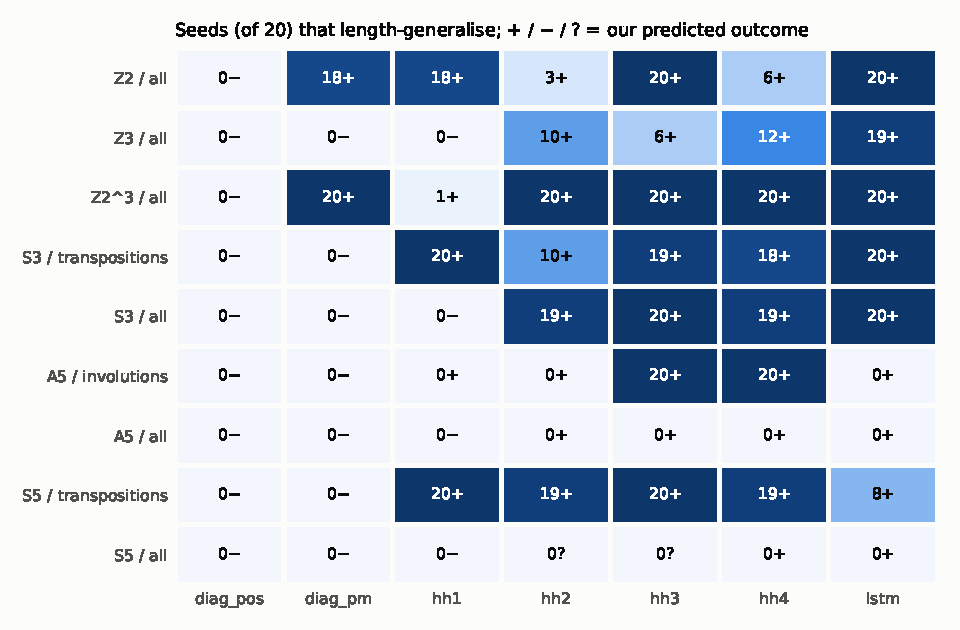
\includegraphics[width=0.78\textwidth]{fig_grid.pdf}\caption{Preregistered grid: number of seeds (out of 20) whose accuracy on positions 257-512 is at least 0.9, with the outcome predicted by the algebraic law (+ success, − failure, ? undetermined). Table 2 is the table view. Claims {[}C-G-*{]}.}\end{figure*}
\begin{figure*}[t]\centering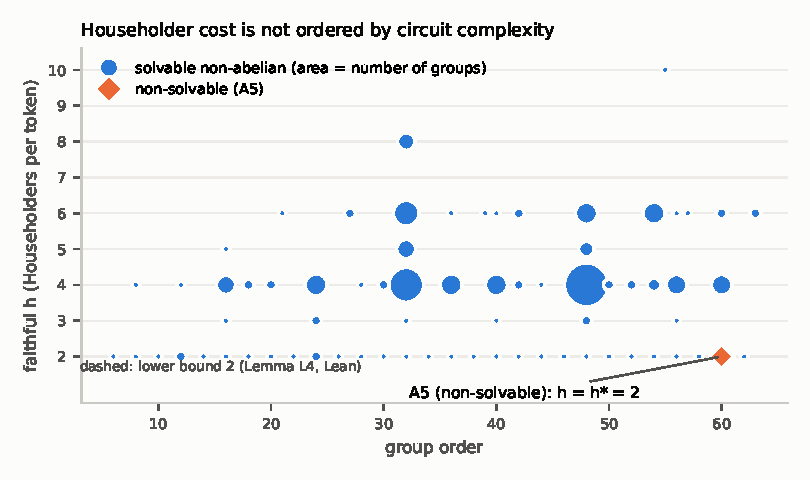
\includegraphics[width=0.78\textwidth]{fig_atlas.pdf}\caption{Atlas of all non-abelian groups of order at most 63: faithful h against group order (dot area = number of groups with that order and h). The only non-solvable group, A5, sits at the minimum value 2 while most solvable groups need more. Claims {[}C-atlas-monotone{]}, {[}C-atlas-nonsolvable{]}.}\end{figure*}
\begin{table*}[t]\centering\small\caption{Certified one-layer Householder complexity (exact verifier). lower: certified lower bound (Lemma L4 for 2); upper: best exact realisation found by the verifier (construction / sign twist, covering-group order |H|, dimension d); h: faithful representations of G only (own and GAP character tables); perm: cost in the permutation representation (the representation law of prior work). Claims [C-T-\textasteriskcentered].}
\begin{tabular}{lllllllllll}\hline
G & alphabet & order & solvable & lower & upper & construction & abs(H) & d & h & perm \\
Z2 & all & 2 & yes & 1 & 1 & perm/none & 2 & 2 & 1 & 1 \\
Z3 & all & 3 & yes & 2 & 2 & perm/none & 3 & 3 & 2 & 2 \\
Z5 & all & 5 & yes & 2 & 2 & planar/none & 5 & 2 & 2 & 4 \\
Z6 & all & 6 & yes & 2 & 2 & planar/none & 6 & 2 & 2 & 5 \\
Z2\^{}2 & all & 4 & yes & 1 & 1 & count/none & 8 & 3 & 2 & 2 \\
Z2\^{}3 & all & 8 & yes & 1 & 1 & count/none & 128 & 7 & 3 & 3 \\
S3 & transpositions & 6 & yes & 1 & 1 & perm/none & 6 & 3 & 1 & 1 \\
S3 & all & 6 & yes & 2 & 2 & perm/none & 6 & 3 & 2 & 2 \\
D4 & all & 8 & yes & 2 & 2 & planar/none & 8 & 2 & 2 & 3 \\
D5 & all & 10 & yes & 2 & 2 & planar/none & 10 & 2 & 2 & 4 \\
Q8 & all & 8 & yes & 2 & 6 & perm/none & 8 & 8 & 4 & 6 \\
A4 & all & 12 & yes & 2 & 2 & perm/none & 12 & 4 & 2 & 2 \\
S4 & transpositions & 24 & yes & 1 & 1 & perm/none & 24 & 4 & 1 & 1 \\
S4 & all & 24 & yes & 2 & 2 & so3/none & 24 & 3 & 2 & 3 \\
S4 & tn & 24 & yes & 2 & 2 & so3/none & 24 & 3 & 2 & 3 \\
A5 & c3c5 & 60 & no & 2 & 2 & so3/none & 60 & 3 & 2 & 4 \\
S5 & tn & 120 & no & 2 & 4 & perm/none & 120 & 5 & 4 & 4 \\
A5 & involutions & 60 & no & 1 & 1 & so3/involutions & 120 & 3 & 2 & 2 \\
A5 & cycles3 & 60 & no & 2 & 2 & perm/none & 60 & 5 & 2 & 2 \\
A5 & cycles5 & 60 & no & 2 & 2 & so3/none & 60 & 3 & 2 & 4 \\
A5 & all & 60 & no & 2 & 2 & so3/none & 60 & 3 & 2 & 4 \\
S5 & transpositions & 120 & no & 1 & 1 & perm/none & 120 & 5 & 1 & 1 \\
S5 & all & 120 & no & 2 & 4 & perm/none & 120 & 5 & 4 & 4 \\\hline
\end{tabular}\end{table*}
\begin{table*}[t]\centering\small\caption{Preregistered grid: successful seeds out of 20 (accuracy >= 0.9 on positions 257-512 of length-512 sequences); mark: predicted success (+), predicted failure (-), undetermined (?) by our predictor. Claims [C-G-\textasteriskcentered].}
\begin{tabular}{llllllll}\hline
task & diag\_pos & diag\_pm & hh1 & hh2 & hh3 & hh4 & lstm \\
Z2/all & 0 - & n/a & n/a & 3 + & 20 + & 6 + & n/a \\
Z3/all & 0 - & n/a & n/a & 10 + & 6 + & 12 + & n/a \\
Z2\^{}3/all & n/a & n/a & n/a & n/a & 20 + & 20 + & n/a \\
S3/transpositions & n/a & n/a & n/a & n/a & n/a & 18 + & n/a \\
S3/all & n/a & n/a & n/a & n/a & n/a & 19 + & n/a \\
A5/involutions & n/a & n/a & n/a & n/a & n/a & 20 + & n/a \\
A5/all & n/a & n/a & n/a & n/a & n/a & 0 + & n/a \\
S5/transpositions & n/a & n/a & n/a & n/a & n/a & 19 + & n/a \\
S5/all & n/a & n/a & n/a & n/a & n/a & 0 + & n/a \\\hline
\end{tabular}\end{table*}
\begin{table*}[t]\centering\small\caption{Preregistered addendum H-EX2: the generator formats of the closest prior work. Successful seeds of 20 at 2x-4x (7x-8x); predicted outcome by our law (h$^*$ = 2 for both tasks) and by the permutation-representation law. Claims [C-X-\textasteriskcentered].}
\begin{tabular}{llllll}\hline
task & model & seeds 2x-4x & seeds 7x-8x & ours & permutation law \\
A5/c3c5 & hh1 & 0 & 0 & failure & failure \\
A5/c3c5 & hh2 & 18 & 18 & success & failure \\
A5/c3c5 & hh3 & 18 & 10 & success & failure \\
S4/tn & hh3 & 19 & 3 & success & success \\\hline
\end{tabular}\end{table*}
\begin{table*}[t]\centering\small\caption{Atlas, all 319 groups of order <= 63, full alphabet. Claims [C-atlas\textasteriskcentered].}
\begin{tabular}{lllll}\hline
class & groups & h$^*$ exact & faithful h = 2 & faithful h >= 3 \\
abelian & 105 & 105 & 62 & 42 \\
solvable non-abelian & 212 & 31 & 31 & 181 \\
non-solvable & 1 & 1 & 1 & 0 \\\hline
\end{tabular}\end{table*}
\onecolumn
\appendix
\section{Claim trace (Appendix C)}
Every statement in the text cites claim identifiers in square brackets. The table lists every claim with its evidence level
(proved\_lean: Lean 4 + Mathlib; computed\_rigorous: exact verifier; statistical: preregistered tests; observed; hypothesis: hand
proof or uninspected interpretation) and the start of its canonical text. Full texts: projects/expressivity/paper\_evidence.json;
proofs of the hand-proved lemmas: expressivity/theory.md (companion ledger).
\begin{scriptsize}\begin{longtable}{@{}
  >{\raggedright\arraybackslash}p{(\linewidth - 6\tabcolsep) * \real{0.2500}}
  >{\raggedright\arraybackslash}p{(\linewidth - 6\tabcolsep) * \real{0.2500}}
  >{\raggedright\arraybackslash}p{(\linewidth - 6\tabcolsep) * \real{0.2500}}
  >{\raggedright\arraybackslash}p{(\linewidth - 6\tabcolsep) * \real{0.2500}}@{}}
\toprule\noalign{}
claim
 & level
 & status
 & canonical text (start)
 \\
\midrule\noalign{}
\bottomrule\noalign{}
C-L1 & proved\_lean & confirmed & Lemma L1 (machine-checked in Lean 4 with Mathlib, theorems rank\_prod\_sub\_one\_le and deltaproduct\_rank\_le): if R\_1, \ldots, R\_k have rank at most one, the\ldots{} \\
C-L4 & proved\_lean & confirmed & Lemma L4 (machine-checked in Lean 4 with Mathlib, theorems sq\_eq\_one\_of\_rank\_le\_one\_of\_pow\_eq\_one and no\_single\_householder\_lift): a real matrix of fi\ldots{} \\
C-L2 & hypothesis & open & Lemma L2 (compression lemma; proved by hand, not machine-checked; reviewed by an independent red-team agent, which found it valid for finite-state rea\ldots{} \\
C-L3 & hypothesis & open & Lemma L3 (sufficiency; proved by hand, and re-verified on every concrete instance by the exact verifier): if a finite group H maps onto G with generat\ldots{} \\
C-thm1 & hypothesis & open & Theorem 1 (from Lemma L2, proved by hand, and Lemma L3): for every finite group G and generating alphabet Sigma, a finite-state one-layer realisation \ldots{} \\
C-L5 & hypothesis & open & Lemma L5 (proved by hand via the compression lemma, not machine-checked; consistent with prior theorems on diagonal SSMs): a finite-state one-layer re\ldots{} \\
C-L7 & hypothesis & open & Lemma L7 (proved by hand; instances certified): for an abelian group h*(G, Sigma) is 1 if every letter is an involution and 2 otherwise; the upper bou\ldots{} \\
C-L6 & observed & confirmed & Computation of h (standard character theory): codim Fix rho(g) = dim rho - (1//g/) sum\_j chi\_rho(g\^{}j), codimensions add over direct sums, and a sum of\ldots{} \\
C-T-Z2-all & computed\_rigorous & confirmed & Certified (Z2, alphabet `all', order 2, 1 letters, solvable): lower bound 1, best certified realisation k = 1 via perm/none (covering group of order 2\ldots{} \\
C-T-Z3-all & computed\_rigorous & confirmed & Certified (Z3, alphabet `all', order 3, 2 letters, solvable): lower bound 2, best certified realisation k = 2 via perm/none (covering group of order 3\ldots{} \\
C-T-Z5-all & computed\_rigorous & confirmed & Certified (Z5, alphabet `all', order 5, 4 letters, solvable): lower bound 2, best certified realisation k = 2 via planar/none (covering group of order\ldots{} \\
C-T-Z6-all & computed\_rigorous & confirmed & Certified (Z6, alphabet `all', order 6, 5 letters, solvable): lower bound 2, best certified realisation k = 2 via planar/none (covering group of order\ldots{} \\
C-T-Z2p2-all & computed\_rigorous & confirmed & Certified (Z2\^{}2, alphabet `all', order 4, 3 letters, solvable): lower bound 1, best certified realisation k = 1 via count/none (covering group of orde\ldots{} \\
C-T-Z2p3-all & computed\_rigorous & confirmed & Certified (Z2\^{}3, alphabet `all', order 8, 7 letters, solvable): lower bound 1, best certified realisation k = 1 via count/none (covering group of orde\ldots{} \\
C-T-S3-transpositions & computed\_rigorous & confirmed & Certified (S3, alphabet `transpositions', order 6, 3 letters, solvable): lower bound 1, best certified realisation k = 1 via perm/none (covering group\ldots{} \\
C-T-S3-all & computed\_rigorous & confirmed & Certified (S3, alphabet `all', order 6, 5 letters, solvable): lower bound 2, best certified realisation k = 2 via perm/none (covering group of order 6\ldots{} \\
C-T-D4-all & computed\_rigorous & confirmed & Certified (D4, alphabet `all', order 8, 7 letters, solvable): lower bound 2, best certified realisation k = 2 via planar/none (covering group of order\ldots{} \\
C-T-D5-all & computed\_rigorous & confirmed & Certified (D5, alphabet `all', order 10, 9 letters, solvable): lower bound 2, best certified realisation k = 2 via planar/none (covering group of orde\ldots{} \\
C-T-Q8-all & computed\_rigorous & confirmed & Certified (Q8, alphabet `all', order 8, 7 letters, solvable): lower bound 2, best certified realisation k = 6 via perm/none (covering group of order 8\ldots{} \\
C-T-A4-all & computed\_rigorous & confirmed & Certified (A4, alphabet `all', order 12, 11 letters, solvable): lower bound 2, best certified realisation k = 2 via perm/none (covering group of order\ldots{} \\
C-T-S4-transpositions & computed\_rigorous & confirmed & Certified (S4, alphabet `transpositions', order 24, 6 letters, solvable): lower bound 1, best certified realisation k = 1 via perm/none (covering grou\ldots{} \\
C-T-S4-all & computed\_rigorous & confirmed & Certified (S4, alphabet `all', order 24, 23 letters, solvable): lower bound 2, best certified realisation k = 2 via so3/none (covering group of order \ldots{} \\
C-T-S4-tn & computed\_rigorous & confirmed & Certified (S4, alphabet `tn', order 24, 2 letters, solvable): lower bound 2, best certified realisation k = 2 via so3/none (covering group of order 24\ldots{} \\
C-T-A5-c3c5 & computed\_rigorous & confirmed & Certified (A5, alphabet `c3c5', order 60, 2 letters, non-solvable): lower bound 2, best certified realisation k = 2 via so3/none (covering group of or\ldots{} \\
C-T-S5-tn & computed\_rigorous & confirmed & Certified (S5, alphabet `tn', order 120, 2 letters, non-solvable): lower bound 2, best certified realisation k = 4 via perm/none (covering group of or\ldots{} \\
C-T-A5-involutions & computed\_rigorous & confirmed & Certified (A5, alphabet `involutions', order 60, 15 letters, non-solvable): lower bound 1, best certified realisation k = 1 via so3/involutions (cover\ldots{} \\
C-T-A5-cycles3 & computed\_rigorous & confirmed & Certified (A5, alphabet `cycles3', order 60, 20 letters, non-solvable): lower bound 2, best certified realisation k = 2 via perm/none (covering group \ldots{} \\
C-T-A5-cycles5 & computed\_rigorous & confirmed & Certified (A5, alphabet `cycles5', order 60, 24 letters, non-solvable): lower bound 2, best certified realisation k = 2 via so3/none (covering group o\ldots{} \\
C-T-A5-all & computed\_rigorous & confirmed & Certified (A5, alphabet `all', order 60, 59 letters, non-solvable): lower bound 2, best certified realisation k = 2 via so3/none (covering group of or\ldots{} \\
C-T-S5-transpositions & computed\_rigorous & confirmed & Certified (S5, alphabet `transpositions', order 120, 10 letters, non-solvable): lower bound 1, best certified realisation k = 1 via perm/none (coverin\ldots{} \\
C-T-S5-all & computed\_rigorous & confirmed & Certified (S5, alphabet `all', order 120, 119 letters, non-solvable): lower bound 2, best certified realisation k = 4 via perm/none (covering group of\ldots{} \\
C-verifier & computed\_rigorous & confirmed & The domain verifier passed its mandatory self-test of 46 known true and known false claims (near-boundary cases such as the same matrices without the \ldots{} \\
C-atlas & computed\_rigorous & confirmed & Atlas over all 319 groups of order at most 63 (GAP SmallGroups library), full alphabet: own numerical character tables and GAP's exact tables give the\ldots{} \\
C-atlas-nonsolvable & computed\_rigorous & confirmed & In the atlas the only non-solvable group is A5 (order 60), with faithful h = 2 and h* = 2 determined exactly\ldots. \\
C-atlas-monotone & computed\_rigorous & confirmed & Non-monotonicity: 181 of the 212 solvable non-abelian groups of order at most 63 have faithful h \textgreater= 3, i.e.~every faithful representation of them need\ldots{} \\
C-atlas-twist & computed\_rigorous & confirmed & Sign lifts to G x Z2 (multiply a letter's matrix by -1) lower the certified upper bound below the faithful h for 37 of the 213 non-abelian groups\ldots. \\
C-atlas-dist & computed\_rigorous & confirmed & Distribution of faithful h over the non-abelian groups of the atlas (value: number of groups): 2: 32, 3: 8, 4: 115, 5: 11, 6: 41, 8: 5, 10: 1\ldots. \\
C-H-protocol & observed & confirmed & Preregistered protocol (prereg.md, committed before the first confirmatory run): one-layer models diag\_pos, diag\_pm, hh1, hh2, hh3, hh4 (DeltaNet/Delt\ldots{} \\
C-G-hh3-Z2-all & statistical & confirmed & Grid cell hh3 on Z2/all: 20 of 20 seeds succeed at 2x-4x the longest training length (18 of 20 at 7x-8x); mean accuracy 0.996 (chance 0.500); in-distr\ldots{} \\
C-G-hh4-Z2-all & statistical & confirmed & Grid cell hh4 on Z2/all: 6 of 20 seeds succeed at 2x-4x the longest training length (7 of 20 at 7x-8x); mean accuracy 0.515 (chance 0.500); in-distrib\ldots{} \\
C-G-hh3-Z3-all & statistical & confirmed & Grid cell hh3 on Z3/all: 6 of 20 seeds succeed at 2x-4x the longest training length (5 of 20 at 7x-8x); mean accuracy 0.444 (chance 0.333); in-distrib\ldots{} \\
C-G-hh4-Z3-all & statistical & confirmed & Grid cell hh4 on Z3/all: 12 of 20 seeds succeed at 2x-4x the longest training length (10 of 20 at 7x-8x); mean accuracy 0.698 (chance 0.333); in-distr\ldots{} \\
C-G-hh3-Z2p3-all & statistical & confirmed & Grid cell hh3 on Z2\^{}3/all: 20 of 20 seeds succeed at 2x-4x the longest training length (0 of 20 at 7x-8x); mean accuracy 0.989 (chance 0.125); in-dist\ldots{} \\
C-G-hh4-Z2p3-all & statistical & confirmed & Grid cell hh4 on Z2\^{}3/all: 20 of 20 seeds succeed at 2x-4x the longest training length (1 of 20 at 7x-8x); mean accuracy 0.981 (chance 0.125); in-dist\ldots{} \\
C-G-hh4-S3-transpositions & statistical & confirmed & Grid cell hh4 on S3/transpositions: 18 of 20 seeds succeed at 2x-4x the longest training length (12 of 20 at 7x-8x); mean accuracy 0.937 (chance 0.167\ldots{} \\
C-G-hh4-S3-all & statistical & confirmed & Grid cell hh4 on S3/all: 19 of 20 seeds succeed at 2x-4x the longest training length (6 of 20 at 7x-8x); mean accuracy 0.971 (chance 0.167); in-distri\ldots{} \\
C-G-hh4-A5-involutions & statistical & confirmed & Grid cell hh4 on A5/involutions: 20 of 20 seeds succeed at 2x-4x the longest training length (0 of 20 at 7x-8x); mean accuracy 0.990 (chance 0.017); i\ldots{} \\
C-G-hh4-A5-all & statistical & confirmed & Grid cell hh4 on A5/all: 0 of 20 seeds succeed at 2x-4x the longest training length (0 of 20 at 7x-8x); mean accuracy 0.017 (chance 0.017); in-distrib\ldots{} \\
C-G-hh4-S5-transpositions & statistical & confirmed & Grid cell hh4 on S5/transpositions: 19 of 20 seeds succeed at 2x-4x the longest training length (11 of 20 at 7x-8x); mean accuracy 0.964 (chance 0.008\ldots{} \\
C-G-hh4-S5-all & statistical & confirmed & Grid cell hh4 on S5/all: 0 of 20 seeds succeed at 2x-4x the longest training length (0 of 20 at 7x-8x); mean accuracy 0.008 (chance 0.008); in-distrib\ldots{} \\
C-H-accuracy & statistical & confirmed & Agreement of each predictor with the cell outcomes on the determined cells: our algebraic predictor 8 of 12; circuit class (solvable) 8 of 12; abelian\ldots{} \\
C-H-NC-hh4-S5 & statistical & confirmed & Preregistered test NC-hh4-S5 (negative control, random targets): cell {[}`hh4', `S5', `all'{]}, successful seeds {[}0{]}, p = 1.000, Benjamini-Hochberg adjust\ldots{} \\
C-H-gates & statistical & confirmed & Preregistered success criteria: accuracy beats every baseline: False; all six discriminating tests significant after BH: False; negative control clean\ldots{} \\
C-expressivity-R2 & computed\_rigorous & confirmed & Lab round 2. Question: For the abelian group Z2\^{}3 with alphabet `all', compare h(Z2\^{}3, all) (faithful representations only) with h*(Z2\^{}3, all). Which \ldots{} \\
C-expressivity-R2-I & hypothesis & open & Uninspected interpretation by the agent for expressivity-R2 (not a result; NOT consistent with the hardened consistency rule): h(Z2\^{}3, all) = 3 (faith\ldots{} \\
C-expressivity-R3 & computed\_rigorous & confirmed & Lab round 3. Question: Liegt h*(A5, involutions) bei 1 oder darüber, wenn man nur ein einzelnes Householder-Produkt pro Token (HH\_1) zulässt, und gilt\ldots{} \\
C-expressivity-R3-I & hypothesis & open & Uninspected interpretation by the agent for expressivity-R3 (not a result; NOT consistent with the hardened consistency rule): \textgreater{} 1\ldots{} \\
C-expressivity-R4 & computed\_rigorous & contested by red-team counter-check & Lab round 4. Question: For the quaternion group Q8 with alphabet `all', what is h(Q8, all), and how far apart are the certified bounds on h*(Q8, all)?\ldots{} \\
C-expressivity-R4-I & hypothesis & open & Uninspected interpretation by the agent for expressivity-R4 (not a result; NOT consistent with the hardened consistency rule): h(Q8, all) = 4\ldots{} \\
C-expressivity-R5 & computed\_rigorous & confirmed & Lab round 5. Question: Can a single layer with 2 Householder reflections per token track the non-solvable group A5 with alphabet `all' exactly? Determ\ldots{} \\
C-expressivity-R5-I & hypothesis & open & Uninspected interpretation by the agent for expressivity-R5 (not a result; consistent with the hardened consistency rule): Ja, 2 Householder-Reflektio\ldots{} \\
C-expressivity-R6 & computed\_rigorous & contested by red-team counter-check & Lab round 6. Question: Wie verhält sich h\emph{(A5, involutions) gegenüber h}(A5, all), wenn man nur die Involutionen als Alphabet zulässt, und ist der Wer\ldots{} \\
C-expressivity-R6-I & hypothesis & open & Uninspected interpretation by the agent for expressivity-R6 (not a result; NOT consistent with the hardened consistency rule): 2\ldots{} \\
C-expressivity-R7 & computed\_rigorous & confirmed & Lab round 7. Question: For S4 with alphabet `all', the permutation representation needs rank(P(s) - I) = 3 for 4-cycles. Is the true h*(S4, all) small\ldots{} \\
C-expressivity-R7-I & hypothesis & open & Uninspected interpretation by the agent for expressivity-R7 (not a result; consistent with the hardened consistency rule): ja, h*(S4, all) = 2\ldots{} \\
C-expressivity-R8 & computed\_rigorous & contested by red-team counter-check & Lab round 8. Question: Welche Gruppen mit Involutionen als Alphabet (z. B. S4, D4, Z2\^{}2 oder Q8 mit geeignetem Twist) besitzen h*(G, involutions) = 1,\ldots{} \\
C-expressivity-R8-I & hypothesis & open & Uninspected interpretation by the agent for expressivity-R8 (not a result; consistent with the hardened consistency rule): Z2\^{}2\ldots{} \\
C-expressivity-R9 & computed\_rigorous & confirmed & Lab round 9. Question: For S5 with alphabet `all', what are the best certified lower and upper bounds on h*(S5, all), and what is h(S5, all) over fait\ldots{} \\
C-expressivity-R9-I & hypothesis & open & Uninspected interpretation by the agent for expressivity-R9 (not a result; NOT consistent with the hardened consistency rule): h*(S5,all): untere Schr\ldots{} \\
C-neg1 & observed & confirmed & Negative result of the lab (no claim passed the verifier and the consistency rule): {[}F3{]} Is one Householder reflection per token (plain DeltaNet with \ldots{} \\
C-lab & observed & confirmed & The agentic lab (literature scout with code-checked quotes, integrator, cascade of four researcher agents, exact verifier, red-team agent, per-round p\ldots{} \\
C-loophole1 & observed & confirmed & Loophole found in lab round 1 and closed: an agent answered `no' (one reflection is not enough for A5 with involution inputs) and backed it with two t\ldots{} \\
C-redteam & observed & confirmed & An independent red-team agent (read and execute only) found three bugs: group names S1, D1, D2 denoted wrong groups (one false sentence each could be \ldots{} \\
C-lit-merrill-tc0 & observed & confirmed & Reference (arXiv:2207.00729, title verified by code against arXiv): ``The Parallelism Tradeoff: Limitations of Log-Precision Transformers''. Verbatim ab\ldots{} \\
C-lit-illusion & observed & confirmed & Reference (arXiv:2404.08819, title verified by code against arXiv): ``The Illusion of State in State-Space Models''. Verbatim abstract quote checked by \ldots{} \\
C-lit-grazzi & observed & confirmed & Reference (arXiv:2411.12537, title verified by code against arXiv): ``Unlocking State-Tracking in Linear RNNs Through Negative Eigenvalues''. Verbatim a\ldots{} \\
C-lit-deltaproduct & observed & confirmed & Reference (arXiv:2502.10297, title verified by code against arXiv): ``DeltaProduct: Improving State-Tracking in Linear RNNs via Householder Products''. \ldots{} \\
C-lit-rwkv7 & observed & confirmed & Reference (arXiv:2503.14456, title verified by code against arXiv): ``RWKV-7''Goose'' with Expressive Dynamic State Evolution''. Verbatim abstract quote \ldots{} \\
C-lit-sarrof & observed & confirmed & Reference (arXiv:2405.17394, title verified by code against arXiv): ``The Expressive Capacity of State Space Models: A Formal Language Perspective''. Ve\ldots{} \\
C-lit-shakerinava & observed & confirmed & Reference (arXiv:2603.01959, title verified by code against arXiv): ``The Expressive Limits of Diagonal SSMs for State-Tracking''. Verbatim abstract quo\ldots{} \\
C-lit-howe & observed & confirmed & Reference (arXiv:2609.18966, title verified by code against arXiv): ``The Automaton Underneath: The Additive Input Pathway Is a Parasitic Attractor for\ldots{} \\
C-lit-liu & observed & confirmed & Reference (arXiv:2210.10749, title verified by code against arXiv): ``Transformers Learn Shortcuts to Automata''. Verbatim abstract quote checked by cod\ldots{} \\
C-lit-cot & observed & confirmed & Reference (arXiv:2310.07923, title verified by code against arXiv): ``The Expressive Power of Transformers with Chain of Thought''. Verbatim abstract qu\ldots{} \\
C-lit-hahn & observed & confirmed & Reference (arXiv:1906.06755, title verified by code against arXiv): ``Theoretical Limitations of Self-Attention in Neural Sequence Models''. Verbatim ab\ldots{} \\
C-lit-deletang & observed & confirmed & Reference (arXiv:2207.02098, title verified by code against arXiv): ``Neural Networks and the Chomsky Hierarchy''. Verbatim abstract quote checked by co\ldots{} \\
C-lit-li-cot & observed & confirmed & Reference (arXiv:2402.12875, title verified by code against arXiv): ``Chain of Thought Empowers Transformers to Solve Inherently Serial Problems''. Verb\ldots{} \\
C-lit-deltaproduct-body & observed & confirmed & Reference arXiv:2502.10297 (full-text quote checked by code against the arXiv HTML): ``Unexpectedly, S 4 and A 5 can extrapolate robustly using only n \ldots{} \\
C-lit-deltaproduct-so3-body & observed & confirmed & Reference arXiv:2502.10297 (full-text quote checked by code against the arXiv HTML): ``This efficiency arises from their isomorphism to subgroups of SO\ldots{} \\
C-lit-howe-law-body & observed & confirmed & Reference arXiv:2609.18966 (full-text quote checked by code against the arXiv HTML): ``the minimal n h that length-generalizes equals the maximal gener\ldots{} \\
C-lit-howe-format-body & observed & confirmed & Reference arXiv:2609.18966 (full-text quote checked by code against the arXiv HTML): ``S 4 (transposition + 4-cycle), A 5 (3-cycle + 5-cycle; all-even)\ldots{} \\
C-lit-rwkv7-swaps-body & observed & confirmed & Reference arXiv:2503.14456 (full-text quote checked by code against the arXiv HTML): ``RWKV-7 can, by Lemma 2 , solve the problem of tracking swaps on \ldots{} \\
C-lit-grazzi-cd-body & observed & confirmed & Reference arXiv:2411.12537 (full-text quote checked by code against the arXiv HTML): ``every n × n orthogonal matrix can be written as a product of n r\ldots{} \\
C-lit-barrington & observed & confirmed & Reference (doi:10.1016/0022-0000(89)90037-8, title verified by code against Crossref): ``Bounded-width polynomial-size branching programs recognize exa\ldots{} \\
\end{longtable}\end{scriptsize}

\end{document}
